%************************************************
\section{Simulation Designer} % (fold)
\label{sec:impl_simulation_designer}
%************************************************
As discussed in Section \ref{sec:simulation_designer}, the Simulation Designer helps the system designer augment the objects she/he wants categorised into SSM Sets during the simulation. It helps to identify and configure these objects with Ego Metadata.\\

First, we present the 3D model formats JME is compatible with. As defined in JME's feature description\footnote{\url{http://jmonkeyengine.org/features/asset-pipeline/}}, JME is compatible with the following 3D model formats:
\begin{itemize}
	\item \emph{.blend} Blender \cite{blender:online} is the most popular open source 3D modelling application. Most major model formats can be imported into Blender, which in turn can be saved as a .blend and used in jME3.
	\item \emph{.ogrexml} OGRE3D is a game rendering engine with a very stable asset pipeline. OgreXML exporter plugins have been written for all major modelling  applications, including 3DS Max\footnote{\url{http://www.autodesk.com/products/autodesk-3ds-max/overview}}, Maya\footnote{\url{http://www.autodesk.com/products/autodesk-maya/overview}}, Softimage\footnote{\url{http://www.autodesk.com/products/autodesk-softimage/overview}}, and Blender \cite{blender:online}.
	\item \emph{.obj} The Wavefront OBJ format is a widespread alternative export format. It doesn't support animations which makes for less complications when dealing with static assets.
\end{itemize}

As it is the most popular open source 3D modelling application, in this project we have used environment models build in Blender. They are discussed in Section \ref{sec:impl_prototype_simulations}. The JME SDK comes with out of the box tooling to import blender models and a scene composer to modify to modify the model. Importing and working with blender models into JME is briefly covered in Section \ref{sec:sd_import_env_model}.\\

A scene is a complete model of an environment. The scene is usually made up by other object models, including terrain, walls, everyday physical objects, etc. JME provides a map called \emph{user data}. This map holds instances of objects mapped to unique String identifiers. Therefore, using this mechanism, we can identify and augment object with Ego Metadata. When trying to attach an instance of the EgocentricContextData to a certain model, the scene composer, using reflection, builds up a visual form, as illustrated in Figure \ref{fig:sd_config_form}, with all properties of the class allowing the system designer to easily configure the metadata properties.\\

To model the \ref{design:object_properties} we have implemented a class called EgocentricContextData. It contains all the properties defined in the design of the metadata. Moreover, in order to add an object in the user data map, it must be \emph{Savable}. This means it must implement the Savable interface from the JME library. This enables the object to be serialized and de-serialized. This is actually how it ends up from the static model into the simulator. The data is saved in a file along with the 3D model. When the model is loaded in the Simulation Runtime, the user data is also read from the file it was saved in and attached to the corresponding objects.\\

The class diagram in Figure \ref{fig:impl_egocentric_context_data} illustrates how the EgocentricContextData is tied to the JME library. The class implements all the attributes we have described in the design of the Ego Metadata. When serialized and de-serialized, the attributes take meaningful default value. Please inspect the source code for the default value each attribute has.
\begin{figure}[H]
	\centering
	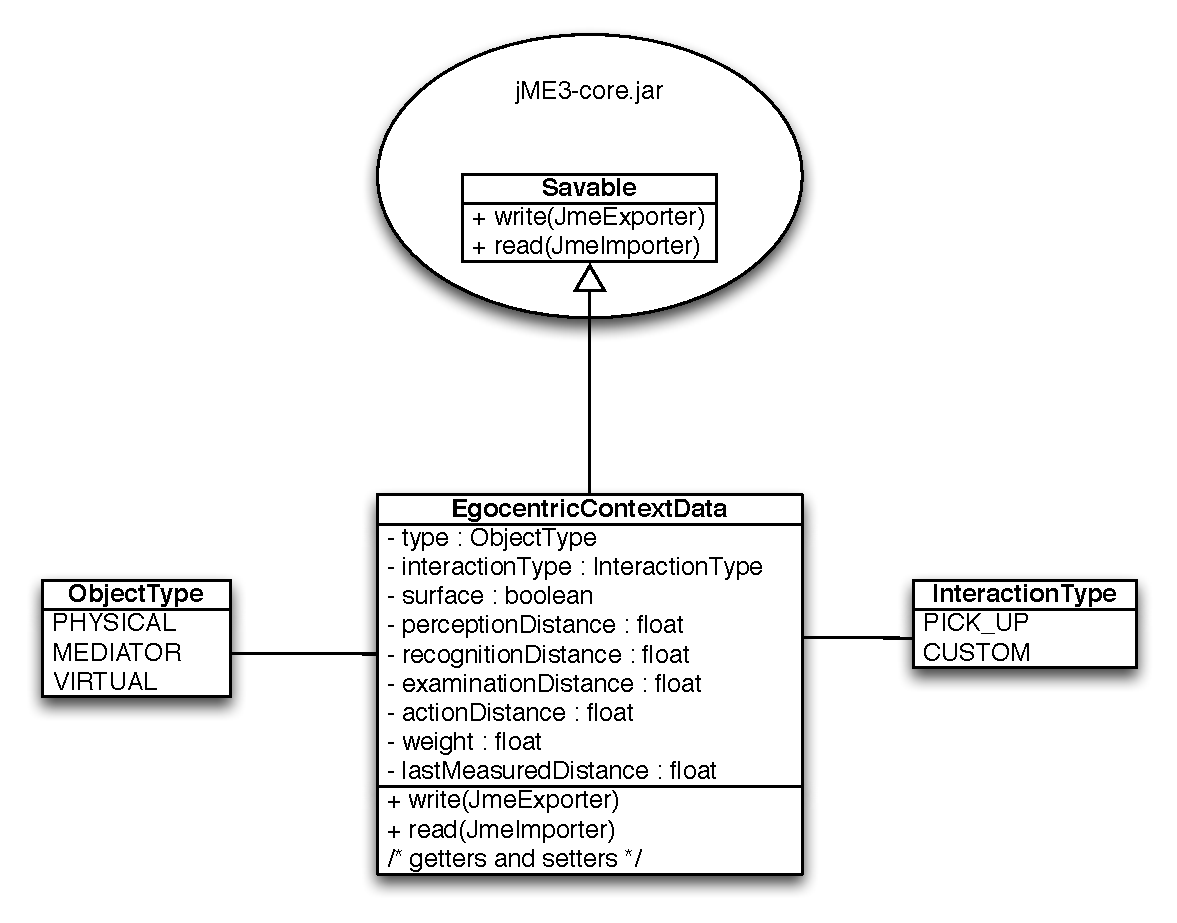
\includegraphics[width=\linewidth]{gfx/Chapter4/ego_metadata}
	\caption{Ego Metadata Class Diagram}
	\label{fig:impl_egocentric_context_data}
\end{figure}

In JME distances are expressed in World Units (WU). This is a subjective interpretation of the distance in real-world metrics, the system designer should decide upon at the time of building the environment.\\

Although we have implemented support to interact with physical objects and devices, we have designed to support virtual objects as well (see the ObjectType enumeration). Moreover, we have designed to support other types of interactions (CUSTOM), except the current pick-up/put-down interaction type (see the InteractionType).\\

When adding EgocentricContextData to an object, always use the ''EGOCENTRIC\_CONTEXT\_DATA'' as the identifier in the user data map. The other components of this framework take into account objects carrying data under this tag. Identifying and augmenting objects to be monitored is covered in Section \ref{sec:sd_identify_objects}.\\

To conclude, Figure \ref{fig:impl_simulation_designer} illustrates a slightly modified design of the simulation designer in the JME context. It is the same design as presented in \ref{fig:final_architecture}, but using components provided by the JME SDK. We have managed to entirely base our configuration process on JME components. Therefore, using the JME Scene Composer from the SDK, the system designer can load a list of supported 3D model formats. Once loaded, the model can be converted to the .j3o format, internal to JME. In the .j3o model the system designer can visually identify the objects he wants monitored augmenting them with the EgocentricContexData information.\\
\begin{figure}[H]
	\centering
	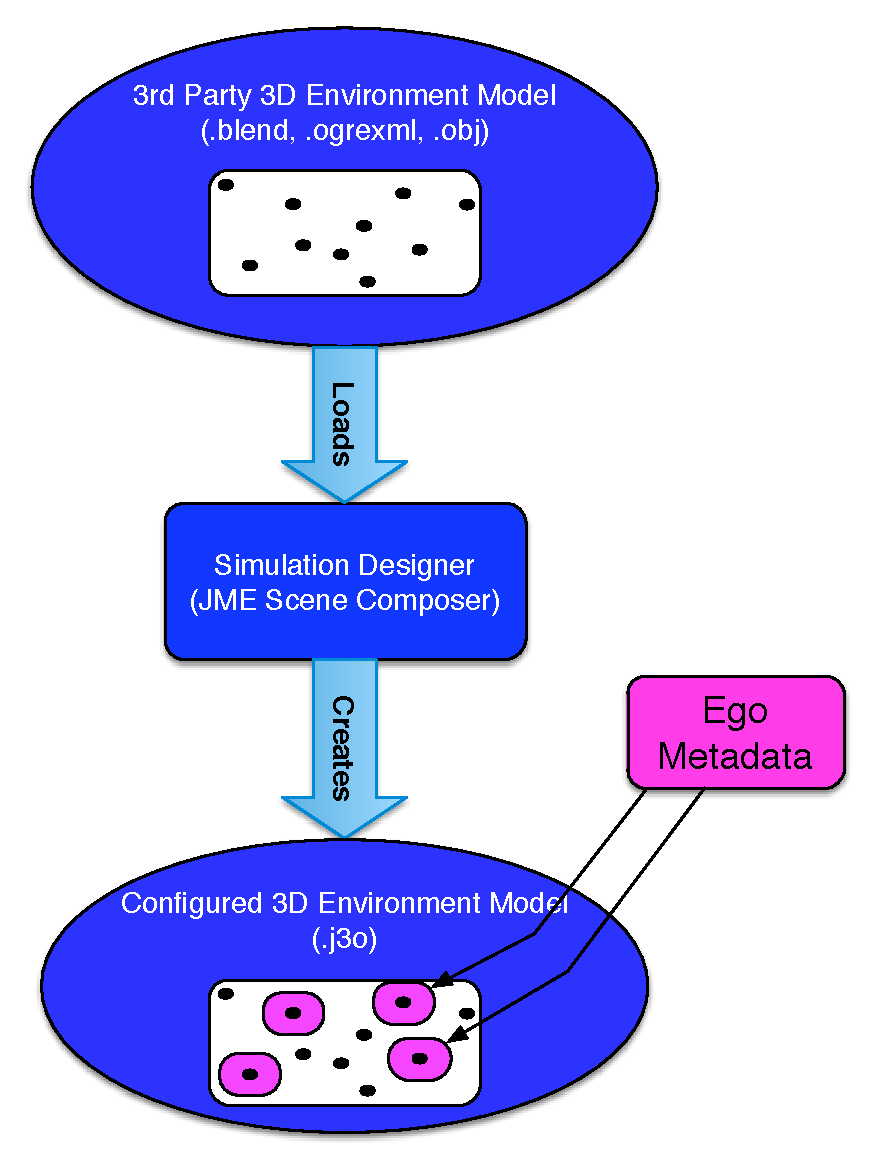
\includegraphics[width=\linewidth]{gfx/Chapter4/simulation_designer}
	\caption{Simulation Designer in the JME context}
	\label{fig:impl_simulation_designer}
\end{figure}
% section impl_simulation_designer (end)